\documentclass[a4paper,12pt]{article}
\usepackage[T1]{fontenc}
\usepackage[utf8]{inputenc}
\usepackage[polish]{babel}
\usepackage{color}
\usepackage{graphicx}
\usepackage{amsmath}
\usepackage{amssymb}
\usepackage{hyperref}
\usepackage{float}
\usepackage{listings}
\usepackage[backend=biber]{biblatex}

\addbibresource{bibliografia.bib}

\lstset{
  basicstyle=\ttfamily,
  columns=flexible,
  keepspaces=true,
  showstringspaces=false,
  escapeinside={(*@}{@*)},
  literate={ą}{{\k{a}}}1
           {ć}{{\'{c}}}1
           {ę}{{\k{e}}}1
           {ł}{{\l{}}}1
           {ń}{{\'{n}}}1
           {ó}{{\'{o}}}1
           {ś}{{\'{s}}}1
           {ź}{{\'{z}}}1
           {ż}{{\.{z}}}1
           {Ą}{{\k{A}}}1
           {Ć}{{\'{C}}}1
           {Ę}{{\k{E}}}1
           {Ł}{{\L{}}}1
           {Ń}{{\'{N}}}1
           {Ó}{{\'{O}}}1
           {Ś}{{\'{S}}}1
           {Ź}{{\'{Z}}}1
           {Ż}{{\.{Z}}}1
           {"}{{\textquotedbl}}1
           {'}{{\textquotesingle}}1
           {`}{{\textasciigrave}}1
           {~}{{\textasciitilde}}1
           {^}{{\textasciicircum}}1
           {_}{{\textunderscore}}1
           {|}{{\textbar}}1
           {\{}{{\textbraceleft}}1
           {\}}{{\textbraceright}}1
           {[}{{[}}1
           {]}{{]}}1
}

\title{4. sprawozdanie z laboratorium Hurtownie Danych}
\author{Mikołaj Kubś, 272662}
\date{\today}

\begin{document}

\maketitle

\begin{enumerate}
    \item DDL (Data Definition Language) - tworzenie struktur danych i schema z użyciem poleceń CREATE, ALTER, DROP
    \item DML (Data Manipulation Language) - manipulacja danymi w tabelach z użyciem poleceń INSERT, UPDATE, DELETE
    \item DCL (Data Control Language) - zarządzanie uprawnieniami, za pomocą poleceń GRANT, DENY, REVOKE
    \item DQL (Data Query Language) - pozyskiwanie danych z bazy, za pomocą polecenia SELECT
\end{enumerate}

\section{Zadanie 1 - przygotowanie schematu}

 {\small
  \begin{lstlisting}[
	language=SQL,
	showspaces=false,
	basicstyle=\ttfamily,
	numbers=left,
	numberstyle=\tiny,
	commentstyle=\color{green},
	tabsize=2
]
CREATE SCHEMA Kubs
\end{lstlisting}}

Utworzenie dedykowanego schematu pozwala na logiczne odseparowanie obiektów stworzonych na potrzeby laboratorium od pozostałych struktur bazy danych.

\section{Zadanie 2 - Tworzenie tabel wymiarów i tabeli faktów}

 {\small
  \begin{lstlisting}[
	language=SQL,
	showspaces=false,
	basicstyle=\ttfamily,
	numbers=left,
	numberstyle=\tiny,
	commentstyle=\color{green},
	tabsize=2
]

CREATE TABLE Kubs.DIM_CUSTOMER (
    CustomerID INT NOT NULL,
    FirstName NVARCHAR(50) NULL,
    LastName NVARCHAR(50) NULL,
    Title NVARCHAR(8) NULL,
    City NVARCHAR(30) NULL,
    TerritoryName NVARCHAR(50) NULL,
    CountryRegionCode NVARCHAR(3) NULL,
    [Group] NVARCHAR(50) NULL
);

CREATE TABLE Kubs.DIM_PRODUCT (
    ProductID INT NOT NULL,
    Name NVARCHAR(50) NOT NULL,
    ListPrice MONEY NULL,
    Color NVARCHAR(15) NULL,
    SubCategoryName NVARCHAR(50) NULL,
    CategoryName NVARCHAR(50) NULL,
    Weight DECIMAL(8, 2) NULL,
    Size NVARCHAR(5) NULL,
    IsPurchased BIT NULL DEFAULT 0
);

CREATE TABLE Kubs.DIM_SALESPERSON (
    SalesPersonID INT NOT NULL,
    FirstName NVARCHAR(50) NULL,
    LastName NVARCHAR(50) NULL,
    Title NVARCHAR(8) NULL,
    Gender NCHAR(1) NULL,
    CountryRegionCode NVARCHAR(3) NULL,
    [Group] NVARCHAR(50) NULL
);

CREATE TABLE Kubs.FACT_SALES (
    ProductID INT NOT NULL,
    CustomerID INT NOT NULL,
    SalesPersonID INT NULL,      
    OrderDate INT NOT NULL,        
    ShipDate INT NULL,             
    OrderQty SMALLINT NOT NULL, 
    UnitPrice MONEY NOT NULL,
    UnitPriceDiscount DECIMAL(8, 4) NOT NULL DEFAULT 0,
    LineTotal DECIMAL(19, 4) NOT NULL
);
\end{lstlisting}}

Zgodnie z poleceniem, kolumny OrderDate oraz ShipDate będą przechowywać dane typu całkowitego.
W tabeli faktów sprzedawca nie jest wymagany.
W tabeli wymiaru dla produktu kategoria i podkategoria również mogą być NULL.
Tabele DIM\_\* pełnią oczywiście role wymiarów, a FACT\_SALES jest tabelą faktów zawierającą miary dotyczące transakcji sprzedaży.

Wartości NULL w niektórych kolumnach wynikają z opcjonalności tych danych w oryginalnym źródle danych lub mogą być nieobecne (również z powodu braku połączenia z inną tabelą, np. produkt bez podkategorii nie może mieć kategorii).


\section{Zadanie 3 - wypełnianie danych}

 {\small
  \begin{lstlisting}[
	language=SQL,
	showspaces=false,
	basicstyle=\ttfamily,
	numbers=left,
	numberstyle=\tiny,
	commentstyle=\color{green},
	tabsize=2
]
INSERT INTO Kubs.DIM_CUSTOMER (
    CustomerID,
    FirstName,
    LastName,
    Title,
    City,
    TerritoryName,
    CountryRegionCode,
    [Group]
)
SELECT DISTINCT
    c.CustomerID,
    p.FirstName,
    p.LastName,
    p.Title,
    a.City,
    st.Name AS TerritoryName,
    st.CountryRegionCode,
    st.[Group]
FROM Sales.Customer AS c
LEFT JOIN Person.Person AS p ON c.PersonID = p.BusinessEntityID
LEFT JOIN Sales.SalesTerritory AS st 
    ON c.TerritoryID = st.TerritoryID
LEFT JOIN Person.BusinessEntityAddress bea 
    ON p.BusinessEntityID = bea.BusinessEntityID 
LEFT JOIN Person.Address AS a ON bea.AddressID = a.AddressID
WHERE c.PersonID IS NOT NULL; 

INSERT INTO Kubs.DIM_PRODUCT (
    ProductID,
    Name,
    ListPrice,
    Color,
    SubCategoryName,
    CategoryName,
    Weight,
    Size,
    IsPurchased
)
SELECT DISTINCT
    p.ProductID,
    p.Name,
    p.ListPrice,
    p.Color,
    psc.Name AS SubCategoryName,
    pc.Name AS CategoryName,
    p.Weight,
    p.Size,
    1 AS IsPurchased
FROM Production.Product AS p
INNER JOIN Sales.SalesOrderDetail AS sod 
    ON p.ProductID = sod.ProductID
LEFT JOIN Production.ProductSubcategory AS psc 
    ON p.ProductSubcategoryID = psc.ProductSubcategoryID
LEFT JOIN Production.ProductCategory AS pc 
    ON psc.ProductCategoryID = pc.ProductCategoryID;

INSERT INTO Kubs.DIM_SALESPERSON (
    SalesPersonID,
    FirstName,
    LastName,
    Title,
    Gender,
    CountryRegionCode,
    [Group]
)
SELECT
    sp.BusinessEntityID AS SalesPersonID,
    p.FirstName,
    p.LastName,
    p.Title,
    e.Gender,
    st.CountryRegionCode,
    st.[Group]
FROM Sales.SalesPerson AS sp
INNER JOIN Person.Person AS p 
    ON sp.BusinessEntityID = p.BusinessEntityID
INNER JOIN HumanResources.Employee AS e 
    ON sp.BusinessEntityID = e.BusinessEntityID
LEFT JOIN Sales.SalesTerritory AS st 
    ON sp.TerritoryID = st.TerritoryID;

INSERT INTO Kubs.FACT_SALES (
    ProductID,
    CustomerID,
    SalesPersonID,
    OrderDate,
    ShipDate,
    OrderQty,
    UnitPrice,
    UnitPriceDiscount,
    LineTotal
)
SELECT
    sod.ProductID,
    soh.CustomerID,
    soh.SalesPersonID,
    DATEPART(YEAR, soh.OrderDate) * 10000 + 
    DATEPART(MONTH, soh.OrderDate) * 100 + 
    DATEPART(DAY, soh.OrderDate) AS OrderDate,
    DATEPART(YEAR, soh.ShipDate) * 10000 + 
    DATEPART(MONTH, soh.ShipDate) * 100 + 
    DATEPART(DAY, soh.ShipDate) AS ShipDate,
    sod.OrderQty,
    sod.UnitPrice,
    sod.UnitPriceDiscount,
    sod.LineTotal
FROM Sales.SalesOrderDetail AS sod
INNER JOIN Sales.SalesOrderHeader AS soh 
    ON sod.SalesOrderID = soh.SalesOrderID;
\end{lstlisting}}

\begin{figure}[H]
    \centering
    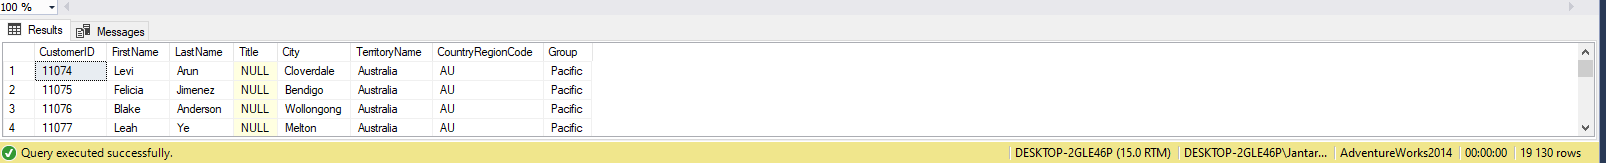
\includegraphics[width=1.0\textwidth]{images/3_customers.png}
    \caption{Pierwsze 3 wiersze DIM\_CUSTOMER i liczba wierszy - 19119}
\end{figure}

\begin{figure}[H]
    \centering
    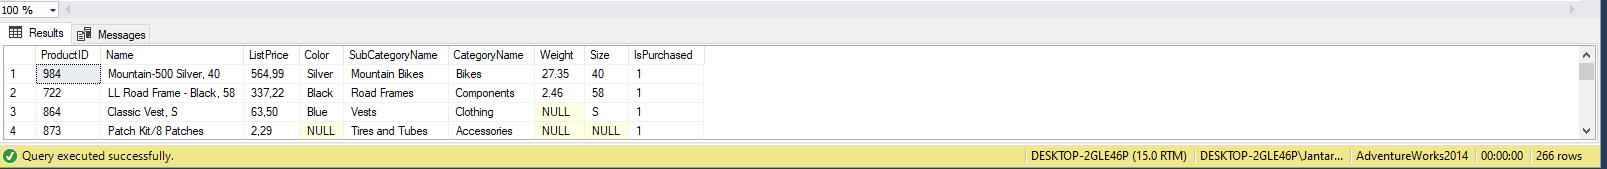
\includegraphics[width=1.0\textwidth]{images/3_products.png}
    \caption{Pierwsze 3 wiersze DIM\_PRODUCT i liczba wierszy - 266}
\end{figure}

\begin{figure}[H]
    \centering
    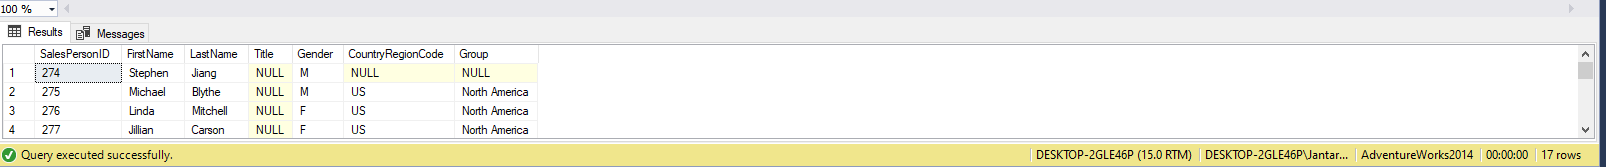
\includegraphics[width=1.0\textwidth]{images/3_sale_people.png}
    \caption{Pierwsze 3 wiersze DIM\_SALESPERSON i liczba wierszy - 17}
\end{figure}

\begin{figure}[H]
    \centering
    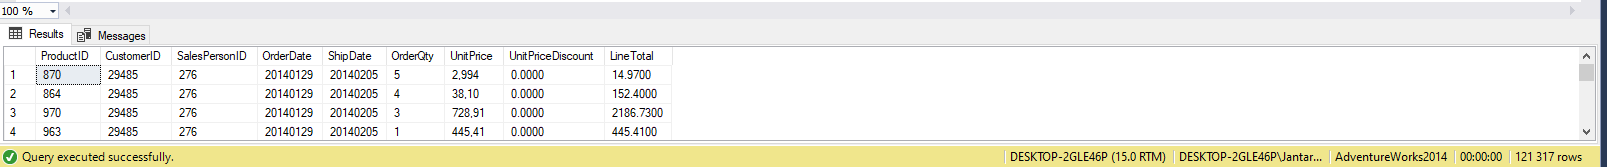
\includegraphics[width=1.0\textwidth]{images/3_sales.png}
    \caption{Pierwsze 3 wiersze FACT\_SALES i liczba wierszy - 121317}
\end{figure}

Zgodnie z poleceniem wypełniono tabele danymi z bazy danych AdventureWorks2014. Ponieważ analizy będą dotyczyć sprzedaży produktów, pominięto wszystkie produkty, które nigdy nie zostały kupione. Okazało się, że wszystkie produkty, które nie miały kategorii lub podkategorii, nigdy nie były kupione.

Liczby wierszy:

DIM\_CUSTOMER - 19119

DIM\_PRODUCT - 266

DIM\_SALESPERSON - 17

FACT\_SALES - 121317

\section{Zadanie 4 - Więzy integralności}

\subsection{Definiowanie kluczy głównych i obcych}

Poniższy kod SQL dodaje klucze główne do tabel wymiarów oraz klucze obce do tabeli faktów, łącząc ją z wymiarami.

    {\small
        \begin{lstlisting}[
    language=SQL,
    showspaces=false,
    basicstyle=\ttfamily,
    numbers=left,
    numberstyle=\tiny,
    commentstyle=\color{green},
    tabsize=2
]
ALTER TABLE Kubs.DIM_CUSTOMER
ADD CONSTRAINT PK_DIM_CUSTOMER PRIMARY KEY (CustomerID);

ALTER TABLE Kubs.DIM_PRODUCT
ADD CONSTRAINT PK_DIM_PRODUCT PRIMARY KEY (ProductID);

ALTER TABLE Kubs.DIM_SALESPERSON
ADD CONSTRAINT PK_DIM_SALESPERSON PRIMARY KEY (SalesPersonID);

ALTER TABLE Kubs.FACT_SALES
ADD CONSTRAINT FK_FACT_SALES_DIM_CUSTOMER
FOREIGN KEY (CustomerID) REFERENCES Kubs.DIM_CUSTOMER(CustomerID);

ALTER TABLE Kubs.FACT_SALES
ADD CONSTRAINT FK_FACT_SALES_DIM_PRODUCT
FOREIGN KEY (ProductID) REFERENCES Kubs.DIM_PRODUCT(ProductID);

ALTER TABLE Kubs.FACT_SALES
ADD CONSTRAINT FK_FACT_SALES_DIM_SALESPERSON
FOREIGN KEY (SalesPersonID) 
    REFERENCES Kubs.DIM_SALESPERSON(SalesPersonID);
\end{lstlisting}
    }

\subsection{Testowanie więzów integralności}

Poniższe instrukcje \texttt{INSERT INTO} mają na celu sprawdzenie działania zdefiniowanych kluczy głównych i obcych. Oczekujemy, że próby wstawienia niepoprawnych danych zakończą się błędami przechwyconymi w blokach \texttt{CATCH}.

{\small
\begin{lstlisting}[
    language=SQL,
    showspaces=false,
    basicstyle=\ttfamily,
    numbers=left,
    numberstyle=\tiny,
    commentstyle=\color{green},
    tabsize=2
]
PRINT 'Test 1: Próba naruszenia PK w DIM_CUSTOMER';
BEGIN TRY
    INSERT INTO Kubs.DIM_CUSTOMER (CustomerID, FirstName, LastName)
    VALUES (11000, 'Test', 'DuplicatePK');

    PRINT 'BŁĄD - duplikat PK';
END TRY
BEGIN CATCH
    PRINT 'SUKCES';
    PRINT ERROR_MESSAGE();
END CATCH
GO

PRINT 'Test 2: Próba naruszenia FK (nieistniejący ProductID) w FACT_SALES';
BEGIN TRY
    INSERT INTO Kubs.FACT_SALES (
        ProductID, CustomerID, SalesPersonID, OrderDate, ShipDate,
        OrderQty, UnitPrice, UnitPriceDiscount, LineTotal
    ) VALUES (
        -999,
        11000,
        NULL,
        20250101, 20250102, 1, 10.0, 0, 10.0
    );

    PRINT 'BŁĄD: Nieistniejące ProductID';
END TRY
BEGIN CATCH
    PRINT 'SUKCES';
    PRINT ERROR_MESSAGE();
END CATCH
GO

PRINT 'Test 3: Próba naruszenia FK (nieistniejący CustomerID) w FACT_SALES';
BEGIN TRY
    INSERT INTO Kubs.FACT_SALES (
        ProductID, CustomerID, SalesPersonID, OrderDate, ShipDate,
        OrderQty, UnitPrice, UnitPriceDiscount, LineTotal
    ) VALUES (
        776,
        -999,
        NULL,
        20240103, 20240104, 2, 20.0, 0, 40.0
    );

    PRINT 'BŁĄD: nieistniejący CustomerID';
END TRY
BEGIN CATCH
    PRINT 'SUKCES';
    PRINT ERROR_MESSAGE();
END CATCH
GO

PRINT 'Koniec testów'
\end{lstlisting}
}

\begin{figure}[H]
    \centering
    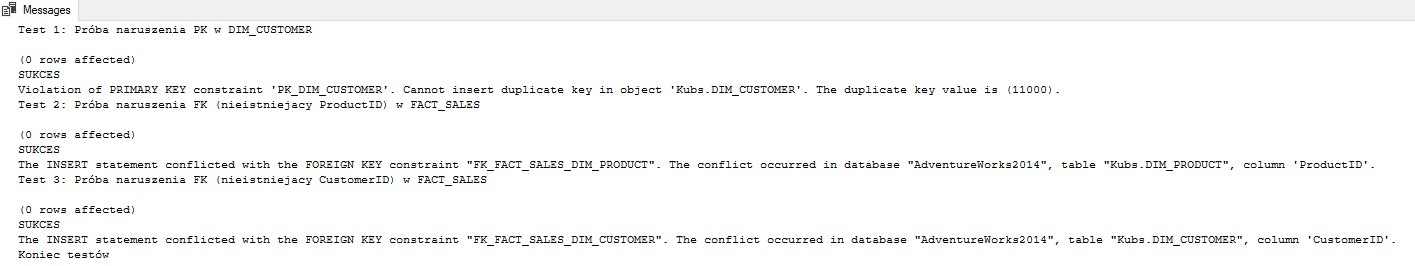
\includegraphics[width=1.0\textwidth]{images/4_2.png}
    \caption{Wykonanie testów więzów integralności}
\end{figure}

Testowe instrukcje zakończyły się przechwyceniem błędów związanych z naruszeniem więzów integralności.

\printbibliography

\end{document}